\documentclass[tikz,border=5pt]{standalone}
\usepackage{fontspec}
\setmainfont{Times New Roman}
\usepackage{unicode-math}
\setmathfont{Cambria Math}
\usetikzlibrary{shapes.geometric,positioning,fit,arrows.meta,calc}

\begin{document}
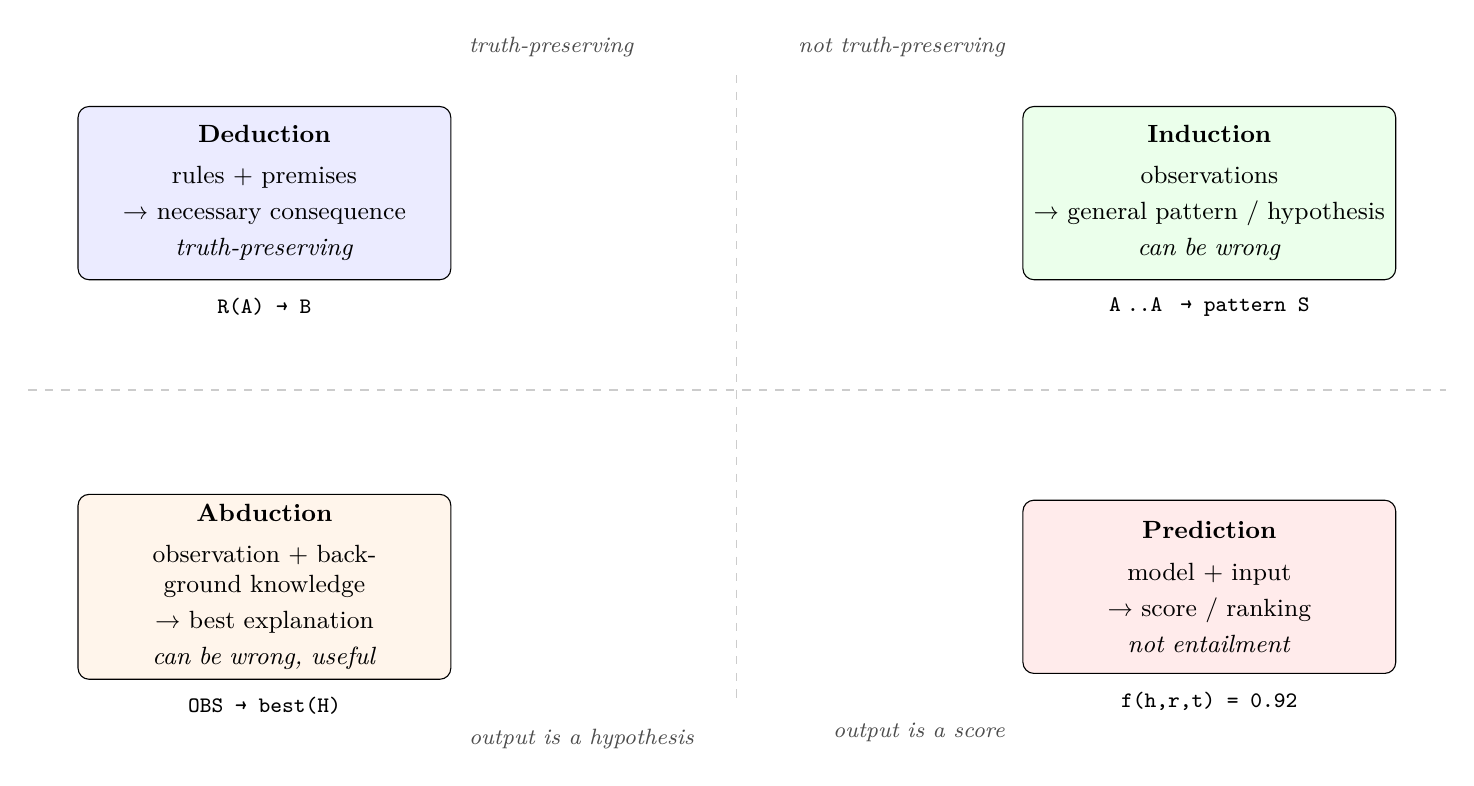
\begin{tikzpicture}[
  box/.style={rectangle, draw, rounded corners, align=center, text width=4.5cm, minimum height=2.2cm, font=\small},
  mono/.style={font=\footnotesize\ttfamily},
  label/.style={font=\footnotesize\itshape},
  arrow/.style={-{Stealth[length=2.5mm]}, thick},
  phase/.style={font=\footnotesize\bfseries},
]

\coordinate (C) at (0,0);

% === Deduction (top-left) ===
\node[box, fill=blue!8] (ded) at (-6, 2.5) {%
  \textbf{Deduction}\\[4pt]
  rules + premises\\[2pt]
  \textrightarrow\ necessary consequence\\[2pt]
  \textit{truth-preserving}
};
\node[mono, below=0.1cm of ded.south] {R(A) → B};

% === Induction (top-right) ===
\node[box, fill=green!8] (ind) at (6, 2.5) {%
  \textbf{Induction}\\[4pt]
  observations\\[2pt]
  \textrightarrow\ general pattern / hypothesis\\[2pt]
  \textit{can be wrong}
};
\node[mono, below=0.1cm of ind.south] {A₁..Aₙ → pattern S};

% === Abduction (bottom-left) ===
\node[box, fill=orange!8] (abd) at (-6, -2.5) {%
  \textbf{Abduction}\\[4pt]
  observation + background knowledge\\[2pt]
  \textrightarrow\ best explanation\\[2pt]
  \textit{can be wrong, useful}
};
\node[mono, below=0.1cm of abd.south] {OBS → best(H)};

% === Prediction (bottom-right) ===
\node[box, fill=red!8] (prd) at (6, -2.5) {%
  \textbf{Prediction}\\[4pt]
  model + input\\[2pt]
  \textrightarrow\ score / ranking\\[2pt]
  \textit{not entailment}
};
\node[mono, below=0.1cm of prd.south] {f(h,r,t) = 0.92};

% === Separators ===
\draw[dashed, gray!40] (0, 4) -- (0, -4);
\draw[dashed, gray!40] (-9, 0) -- (9, 0);

% === Axis labels ===
\node[label, text=gray!60!black, above right=0.5cm and 0.1cm of ded.north east] {truth-preserving};
\node[label, text=gray!60!black, above left=0.5cm and 0.1cm of ind.north west] {not truth-preserving};
\node[label, text=gray!60!black, below right=0.5cm and 0.1cm of abd.south east] {output is a hypothesis};
\node[label, text=gray!60!black, below left=0.5cm and 0.1cm of prd.south west] {output is a score};

\end{tikzpicture}
\end{document}